\chapter{Similar case retrieval for DR diagnosis} \label{chapter6}
In this section we explore another way of using the model in a clinical context beyond mere DR grading: showing the clinician images with similar diagnostic features to help them diagnose a new case. The contents of this section were developed in cooperation with the director of this work, Professor Antonio Alejandro Sánchez Ruiz-Granados, as a part of an article for the International Conference on Case-Based Reasoning. 

\section{Extraction of \textit{embeddings}}
An important part of the expressiveness of neural networks comes from their ability to create low-dimensional representations of the data containing most of the information necessary for the task at hand; these representations are called \textit{embeddings}. Indeed, the output of the global average pooling of the convolutional component of the network (which is a real vector with 1.536 components) must contain most the information necessary to evaluate the DR grading of the image, since this is all the information the classifier is fed. 

In a model like the one depicted in \Cref{fig:architecture}, the classifier is a purely linear component, so different classes must lie in linearly separable components of the space: this means we can use the spatial structure of the embeddings to obtain semantic information about the fundus images.

\begin{figure}[tb]
    \centering
    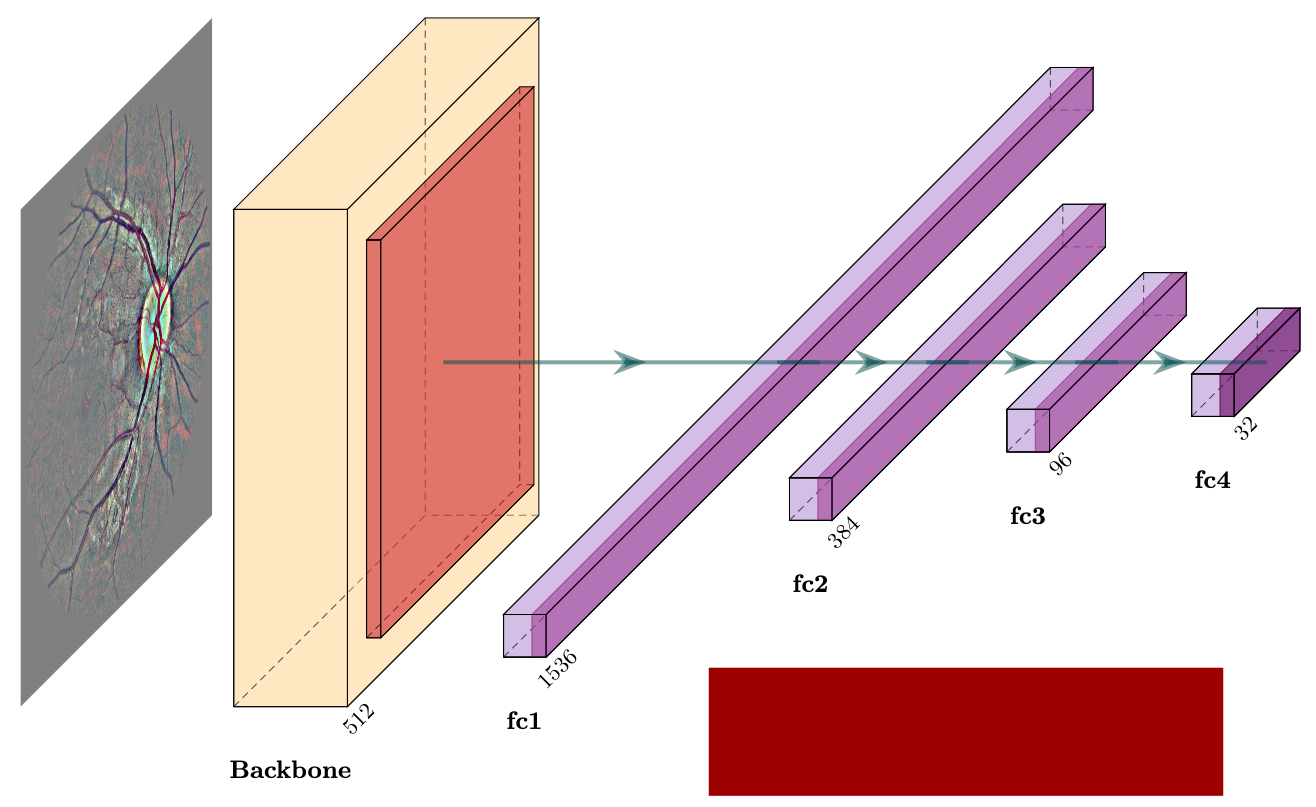
\includegraphics[scale=0.2]{figures/chapter6/model_head.png}
    \caption{Structure of the model after adding a new multilevel classifier. The first two layers are regularized using dropout (\( p = 0.3\)). All the layers use Leaky ReLU (\( \alpha = 0.5 \)) except for the last one, that is purely linear. }
    \label{fig:model_headed}
\end{figure}

However, we found that these embeddings were too high dimensional to be used efficiently and applying generic dimensionality reduction techniques (UMAP, t-SNE or PCA) returned low-quality results. To overcome this problem we extended the classifier adding three regularized fully connected layers (\Cref{fig:model_headed}), serving as a context-aware dimensionality reduction of data. We chose to progressively reduce the width of layers by a factor of \( 4 \), so we had access to embeddings of different dimensionality. In order to save computational power, we reused the convolutional block and retrained the new layers.

In order to visualize embeddings we extracted the input of the \texttt{fc4} layer to obtain 32-dimensional features. Since this is the final linear layer,  these embeddings preserve the aforementioned property of linear separability by class. Extracting the input of previous layers gives us access to additional embeddings for each image, of dimensions 1536, 384 and 96. 

\Cref{fig:embedding}, shows a visualization of the 32-dimensional embeddings for a sample of 3,000 points, projected to the plane using UMAP \cite{mcinnes2018umap} and labelled both by predicted and target class. The image leads us to two relevant assertions: \begin{enumerate*}[label=(\arabic*)]
\item the network successfully creates a representation of the input image that spatially encodes diagnostic information of the disease and \item the spatial structure is robust enough to persist after severe dimensionality reduction\end{enumerate*}. 

\begin{figure}[tb]
     \centering
     \begin{subfigure}[b]{0.49\textwidth}
         \centering
         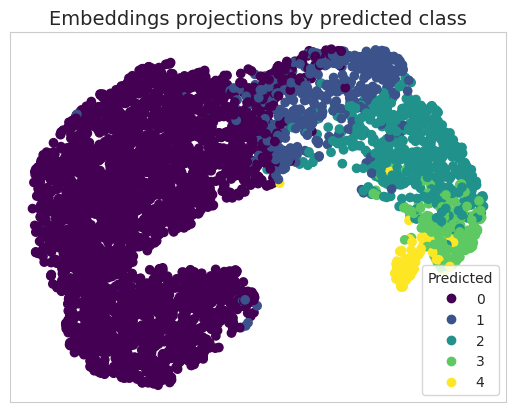
\includegraphics[width=\textwidth]{figures/chapter6/embeddings/embeddings_predicted.png}
         \caption{Embeddings by predicted class}
         \label{fig:embedding_predicted}
     \end{subfigure}
     \hfill
     \begin{subfigure}[b]{0.49\textwidth}
         \centering
         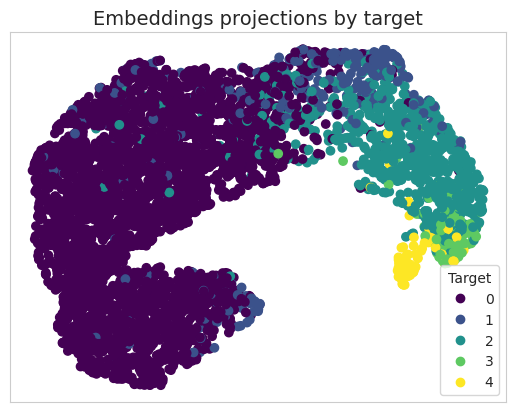
\includegraphics[width=\textwidth]{figures/chapter6/embeddings/embeddings_target.png}
         \caption{Embeddings by target class}
         \label{fig:embedding_target}
    \end{subfigure}
    \caption{Projection into the plane of the 32-dimensional features using UMAP. }
    \label{fig:embedding}
\end{figure}

\begin{figure}[tb]
     \centering
     \begin{subfigure}[b]{0.49\textwidth}
        \centering
        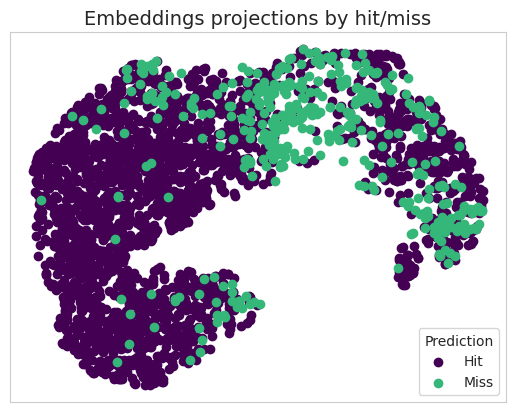
\includegraphics[width=\textwidth]{figures/chapter6/embeddings/hit_miss.png}
        \caption{Projected embeddings labelled by hit/miss on the original image (DR grade was correctly predicted)}
        \label{fig:hit_miss}
     \end{subfigure}
     \hfill
     \begin{subfigure}[b]{0.49\textwidth}
        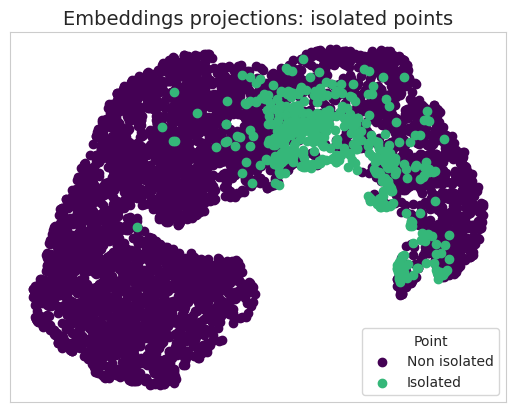
\includegraphics[width=\textwidth]{figures/chapter6/embeddings/isolated.png}
        \caption{Projected embeddings labelled by isolation (distance to the closest point is over two standard deviations of the average distance)}
        \label{fig:isolated}
     \end{subfigure}
     \hfill
    \caption{Projections of the embeddings of a sample (N = 5,000) from the train dataset, labelled by hit/miss and isolation}
    \label{fig:embeddings_explore}
    \centering
\end{figure}


\Cref{fig:hit_miss} explores the distribution of embeddings of wrongly predicted images. These images concentrate over some small regions of the space of the embeddings, which can be used to classify ``high risk'' areas, where the performance of the model may be suboptimal. Interestingly, these zones mostly coincide with the areas of distribution of isolated points (\Cref{fig:isolated}), characterized as those points which distance to the closest point is over two standard deviations the average one. 

In order to further test our assertions, we implemented a k-NN classifier using the 96-dimensional embeddings and different metrics. The class is obtained as the weighted average of the neighbors, weighted by the inverse of the distance. 

The results, shown in \Cref{table:knn}, are impressively solid, achieving even a higher accuracy than the neural network for some choices of \( k \) and a reasonable value for Cohen's \( \kappa \). The results are robust between metrics and choices of \( k \) but using other dimensions for the embeddings severely degraded performance, which reinforces the importance of using adequately sized embeddings for each task. 

\begin{table}[tb]
    \centering
    \small
    \begin{tabular}{c|cccccc|}
    \cline{2-7}
        & \multicolumn{2}{c|}{k = 3} & \multicolumn{2}{c|}{k = 11} & \multicolumn{2}{c|}{k = 15} \\ \cline{2-7} 
        & Accuracy & \multicolumn{1}{c|}{$\kappa$} & Accuracy & \multicolumn{1}{c|}{$\kappa$} & Accuracy & \multicolumn{1}{c|}{$\kappa$} \\ \hline \hline
    \multicolumn{1}{|c|}{Manhattan} & 0.8322 & \multicolumn{1}{c|}{0.7810} & 0.8437 & \multicolumn{1}{c|}{0.7945} & 0.8439 & 0.6078 \\ \hline
    \multicolumn{1}{|c|}{Euclidean} & 0.8324 & \multicolumn{1}{c|}{0.7825} & 0.8439 & \multicolumn{1}{c|}{0.7951} & 0.8440 & 0.6084 \\ \hline
    \multicolumn{1}{|c|}{Cosine} & 0.8336 & \multicolumn{1}{c|}{0.7840} & 0.8431 & \multicolumn{1}{c|}{0.7958} & 0.8425 & 0.6059 \\ \hline
    \end{tabular}
    \caption{Results obtained by a k-NN classifier ($k = 11$) on 96-dimensional embeddings}
\label{table:knn}
\end{table}

We can use the fact that the spatial structure of the embeddings contains diagnostic information to model \textit{semantic search}, the retrieval of images with similar diagnostic signs to a given one, as a \textit{nearest neighbor search} problem.

\begin{figure}[tb]
    \captionsetup[subfigure]{labelformat=empty}
     \centering
     \begin{subfigure}[b]{\textwidth}
        \begin{subfigure}[b]{0.32\textwidth}
            \centering
            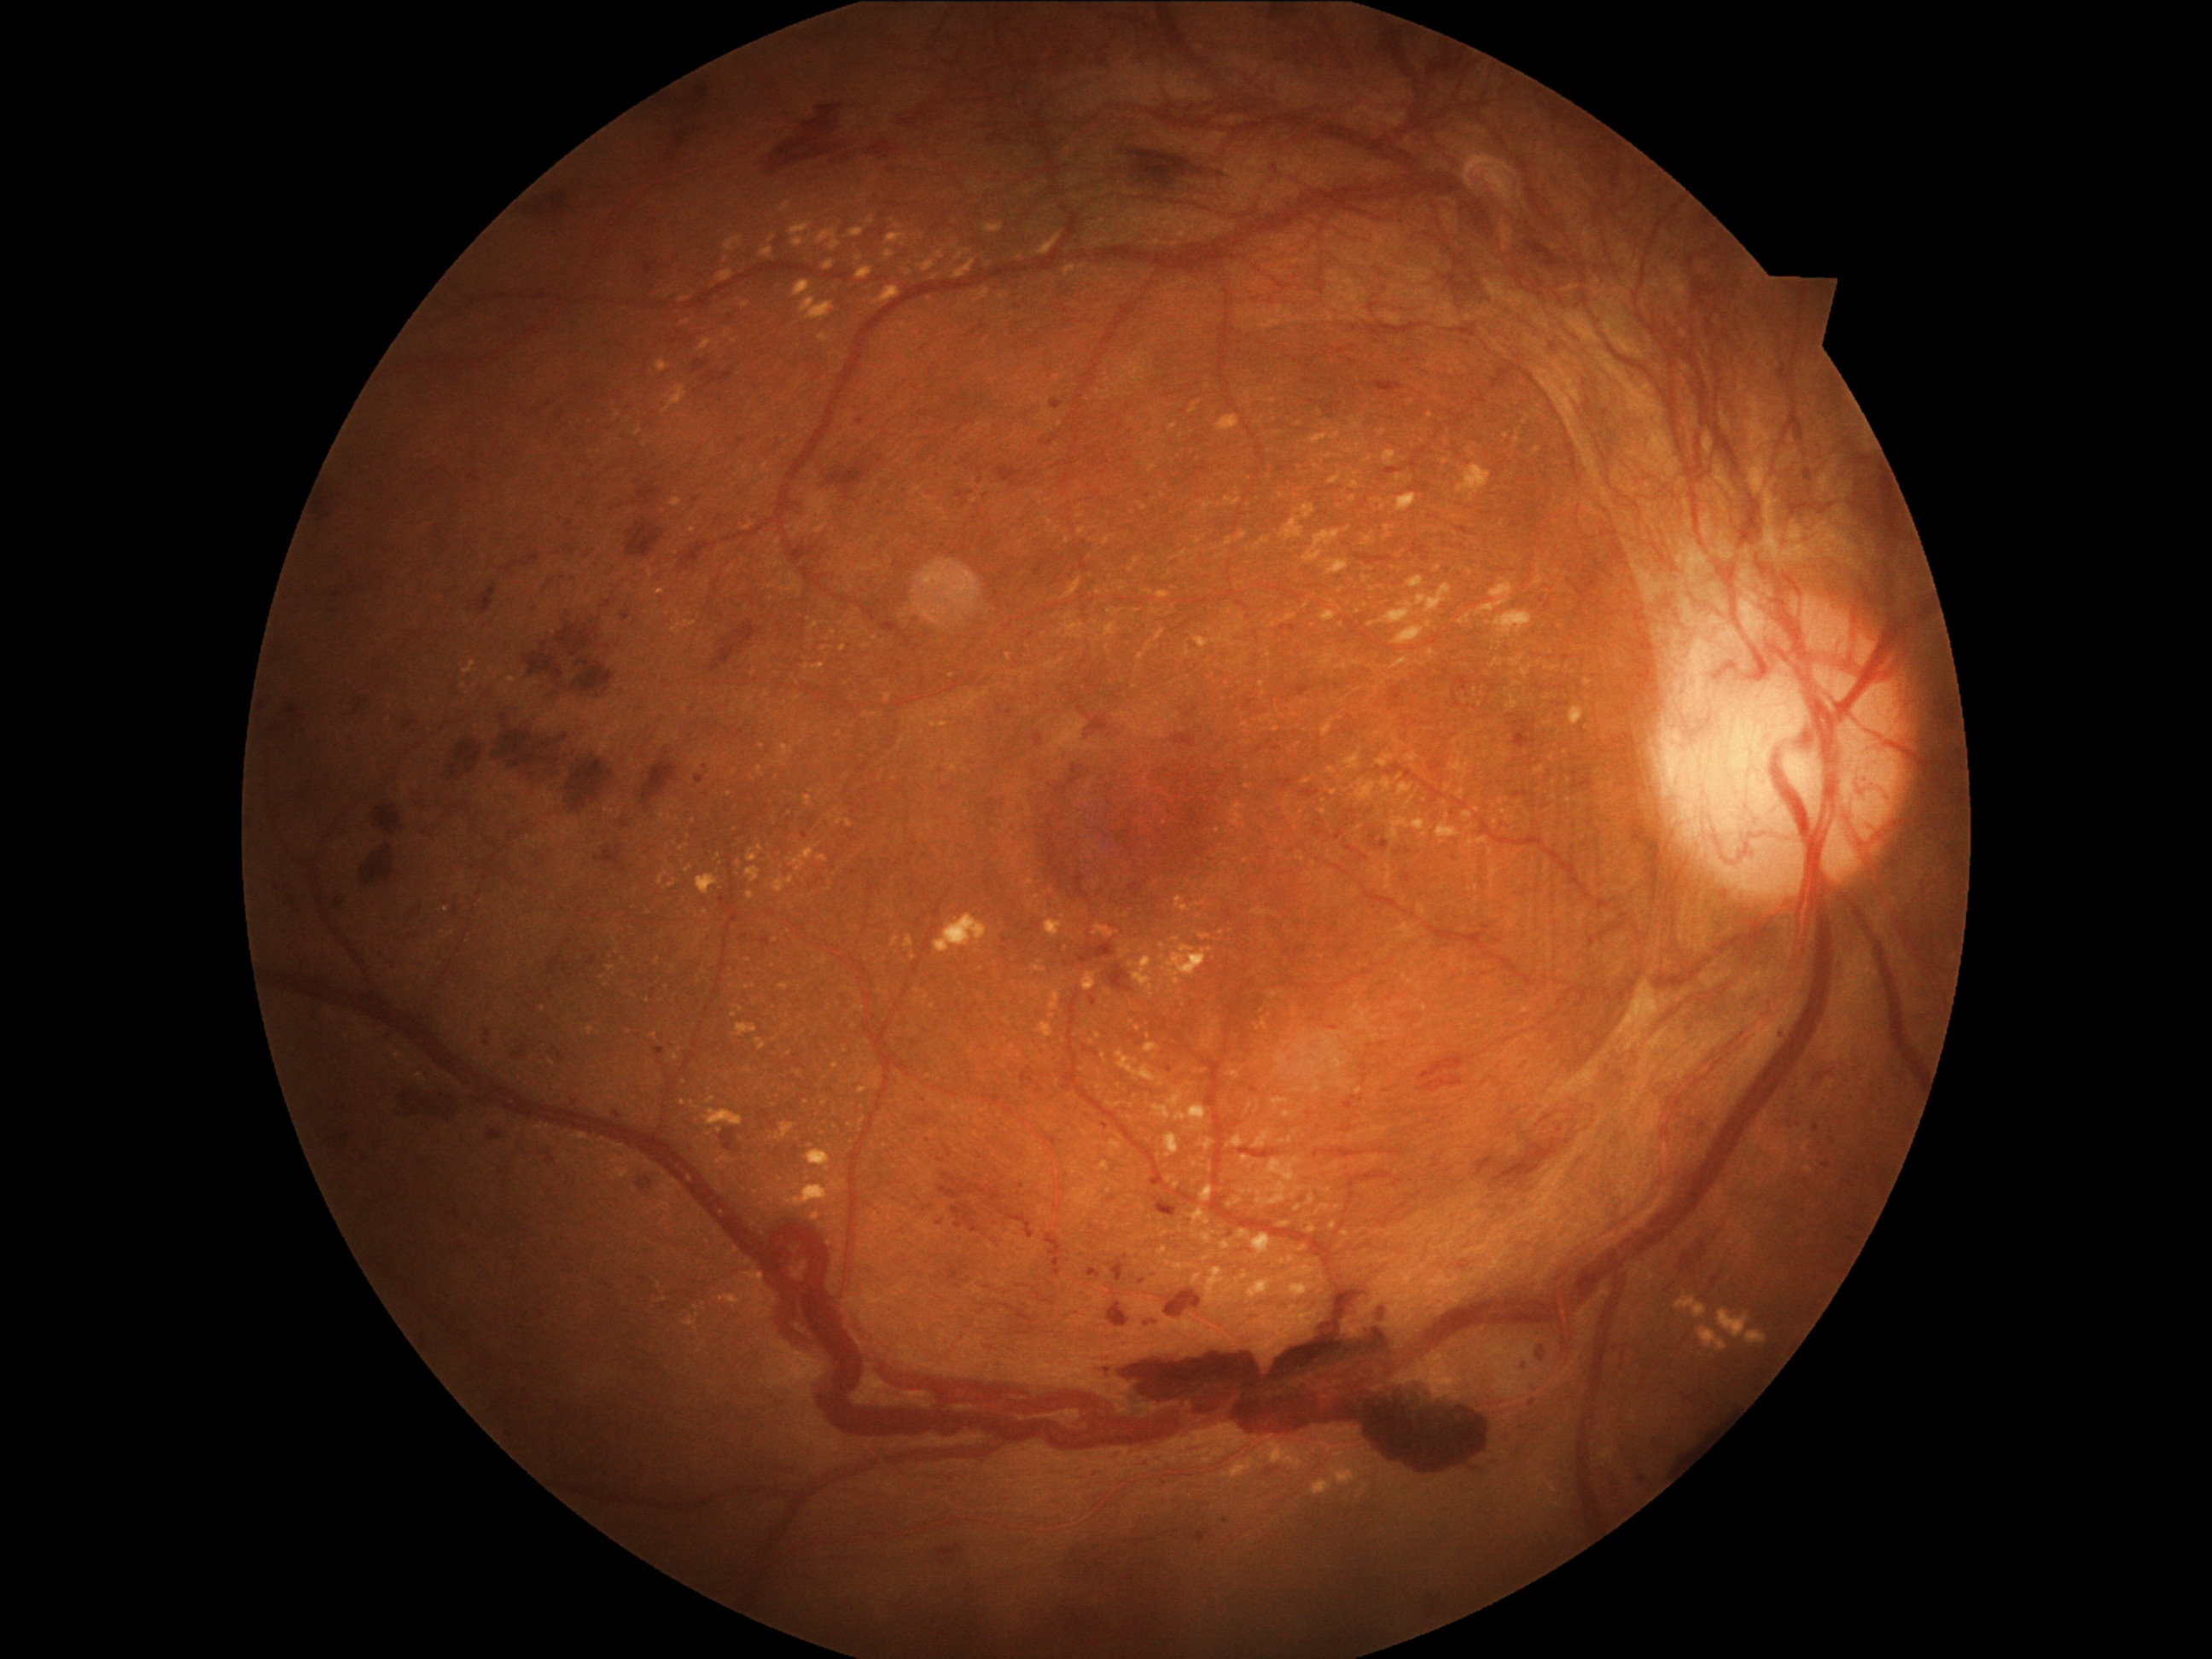
\includegraphics[width=\textwidth, height=0.2\textheight]{figures/chapter6/similar/16473_right.jpeg}
            \caption{Grade 4}
         \end{subfigure}
         \hfill
         \begin{subfigure}[b]{0.32\textwidth}
            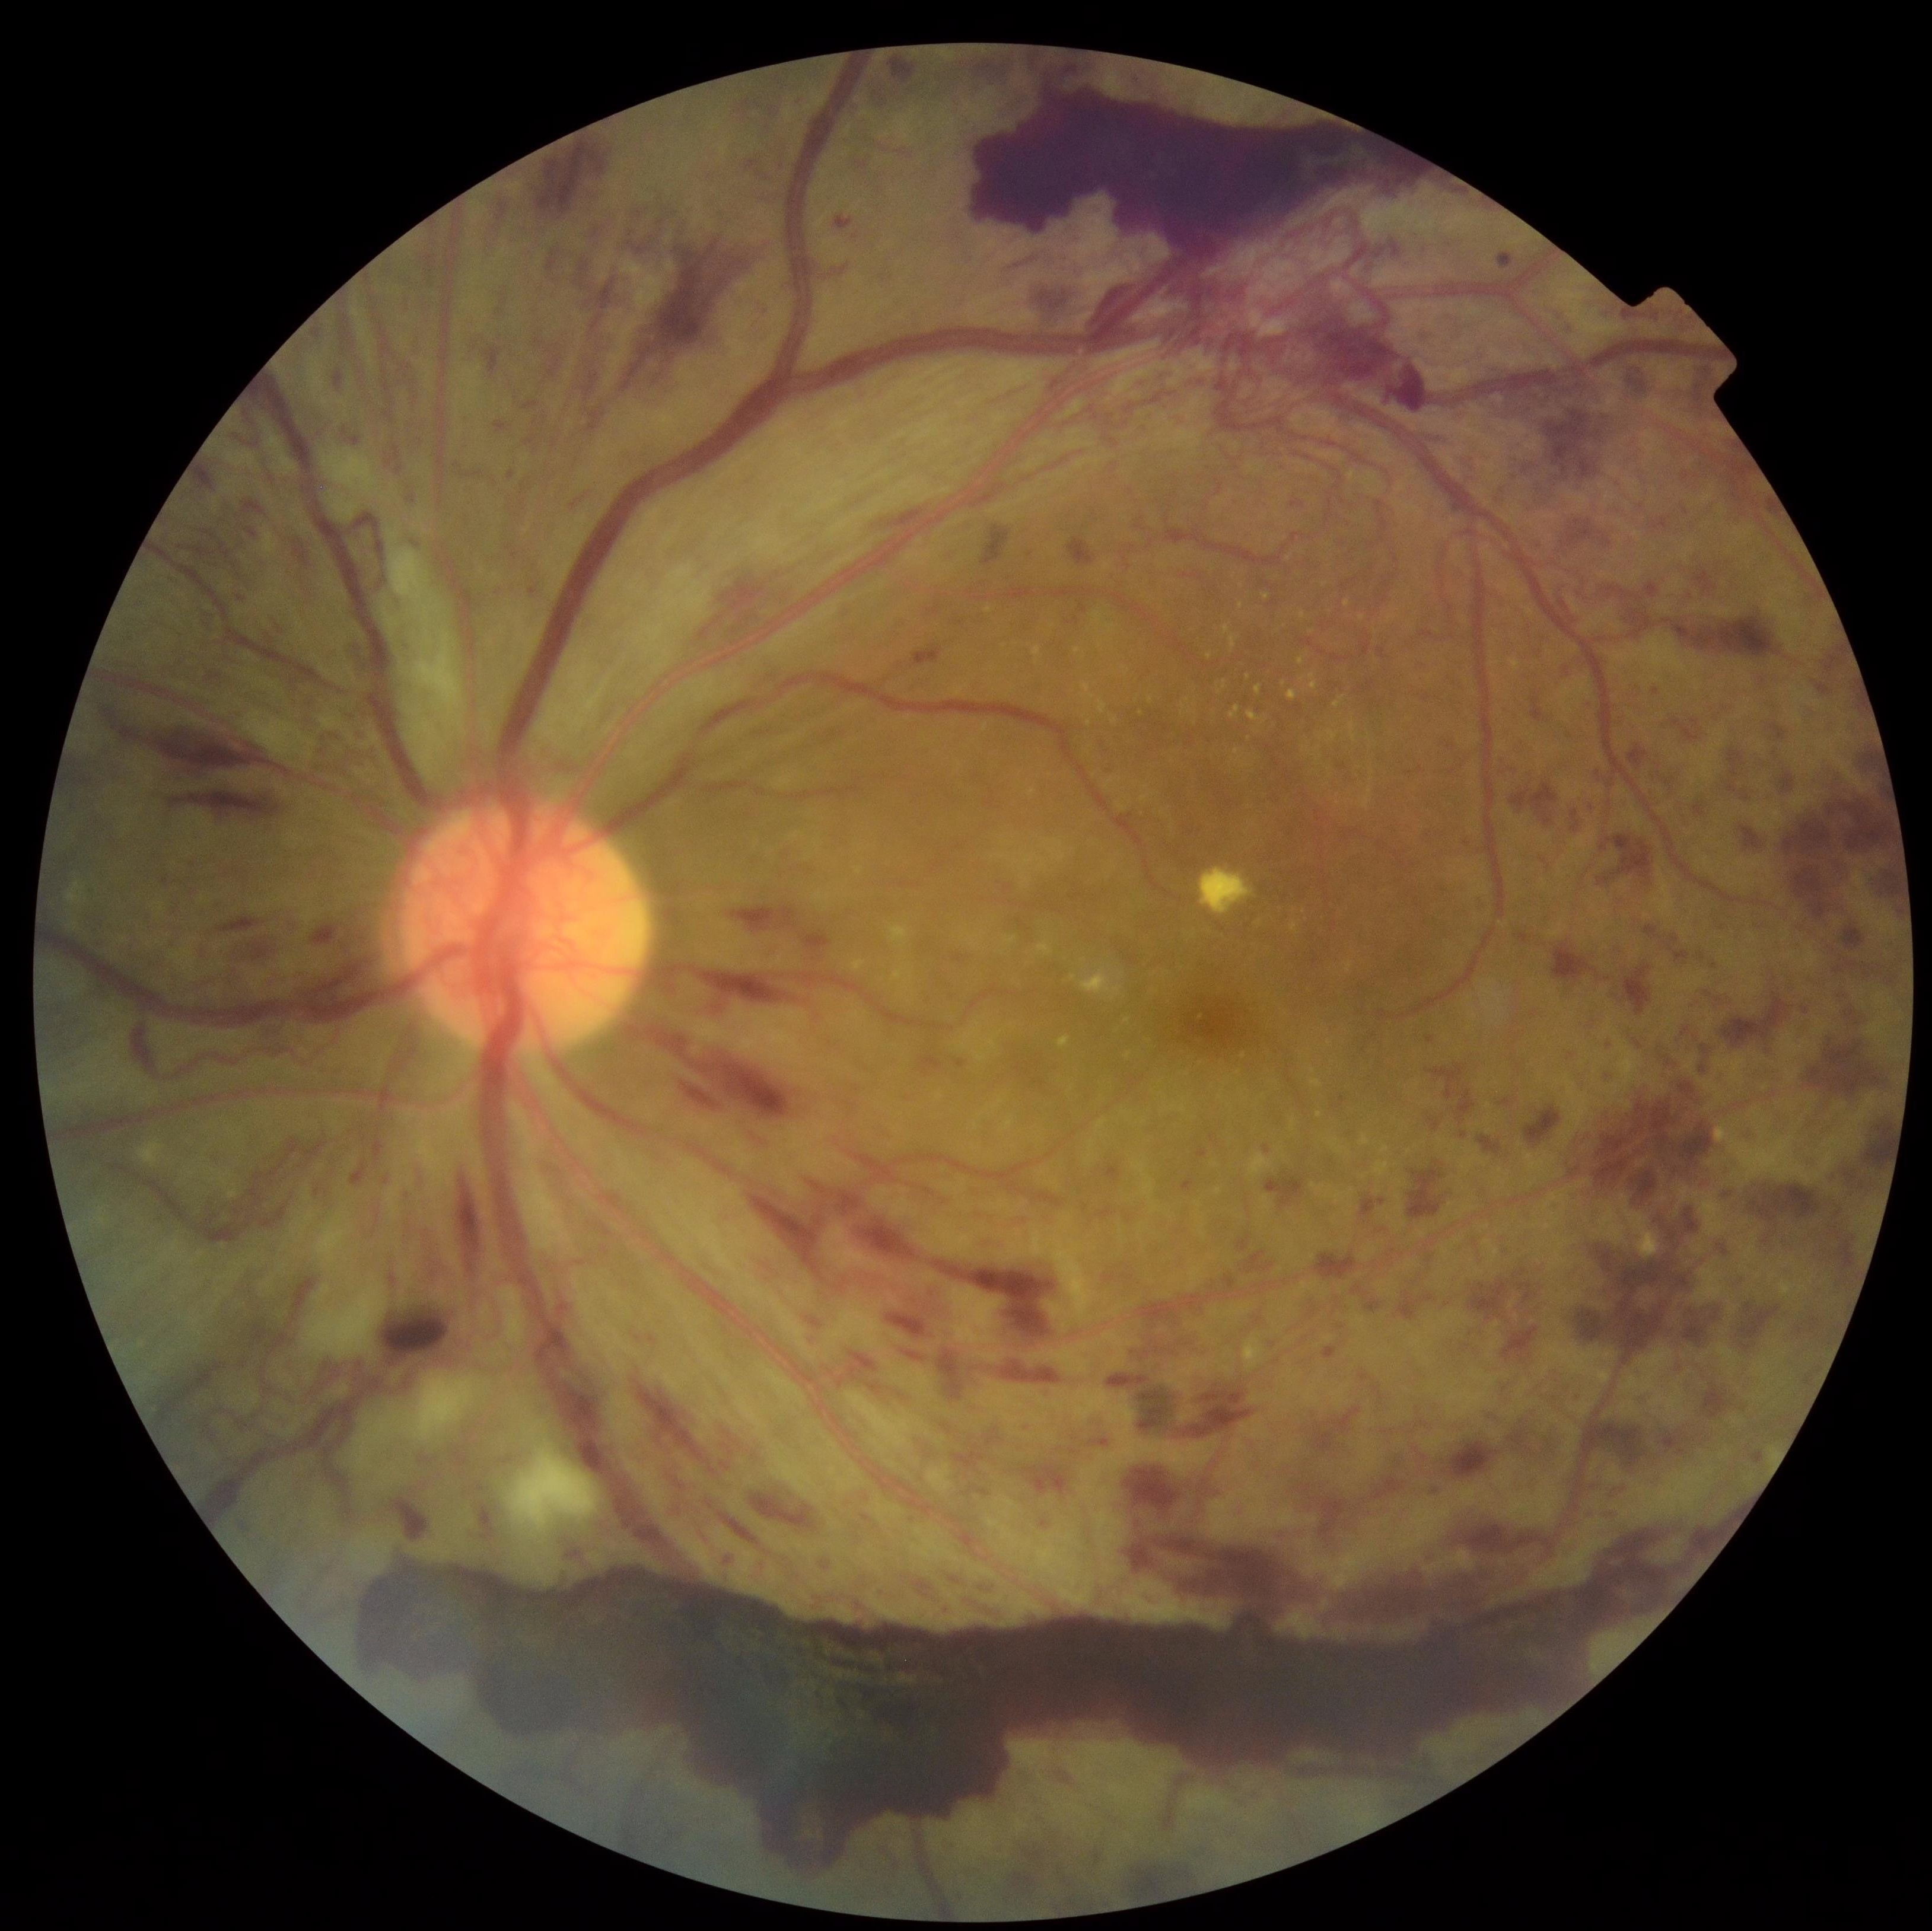
\includegraphics[width=\textwidth, height=0.2\textheight]{figures/chapter6/similar/15975_left.jpeg}
            \caption{Grade 4}
        \end{subfigure}
        \hfill
        \begin{subfigure}[b]{0.32\textwidth}
            \centering
            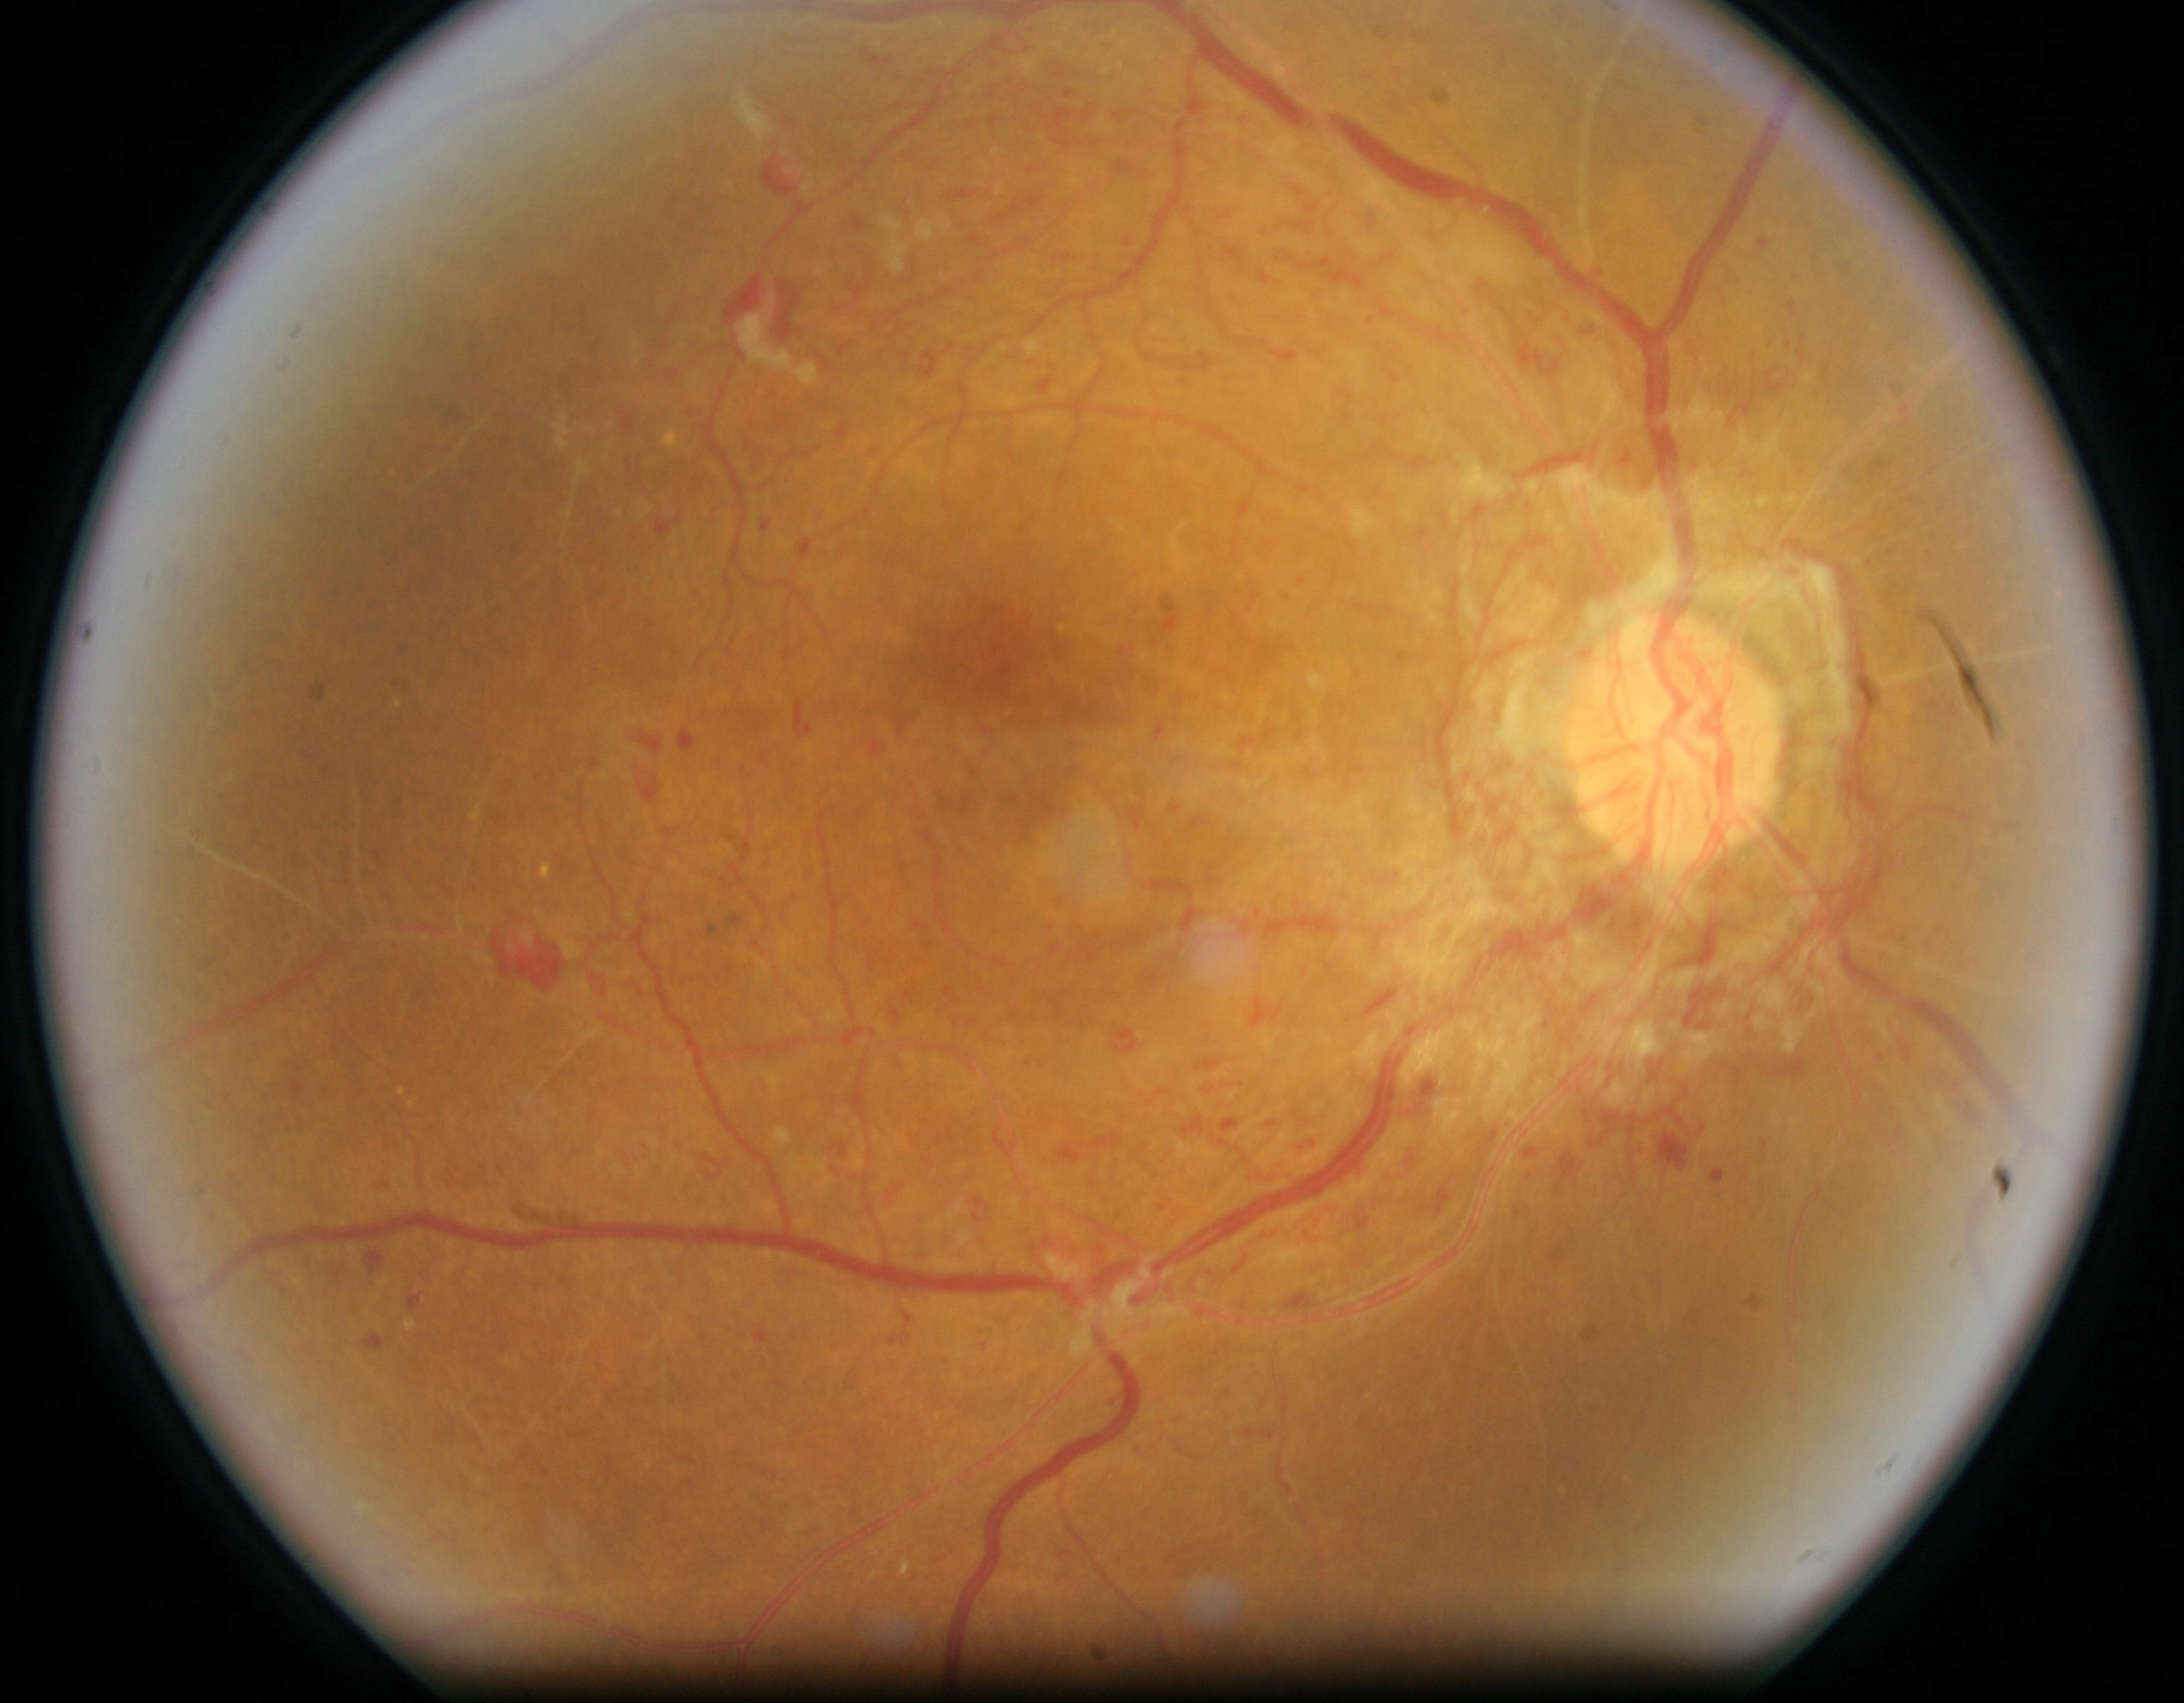
\includegraphics[width=\textwidth, height=0.2\textheight]{figures/chapter6/similar/3563_left.jpeg}
            \caption{Grade 4}
         \end{subfigure}
    \end{subfigure}
    \vspace{0.2em}
    
    \begin{subfigure}[b]{\textwidth}
        \begin{subfigure}[b]{0.32\textwidth}
            \centering
            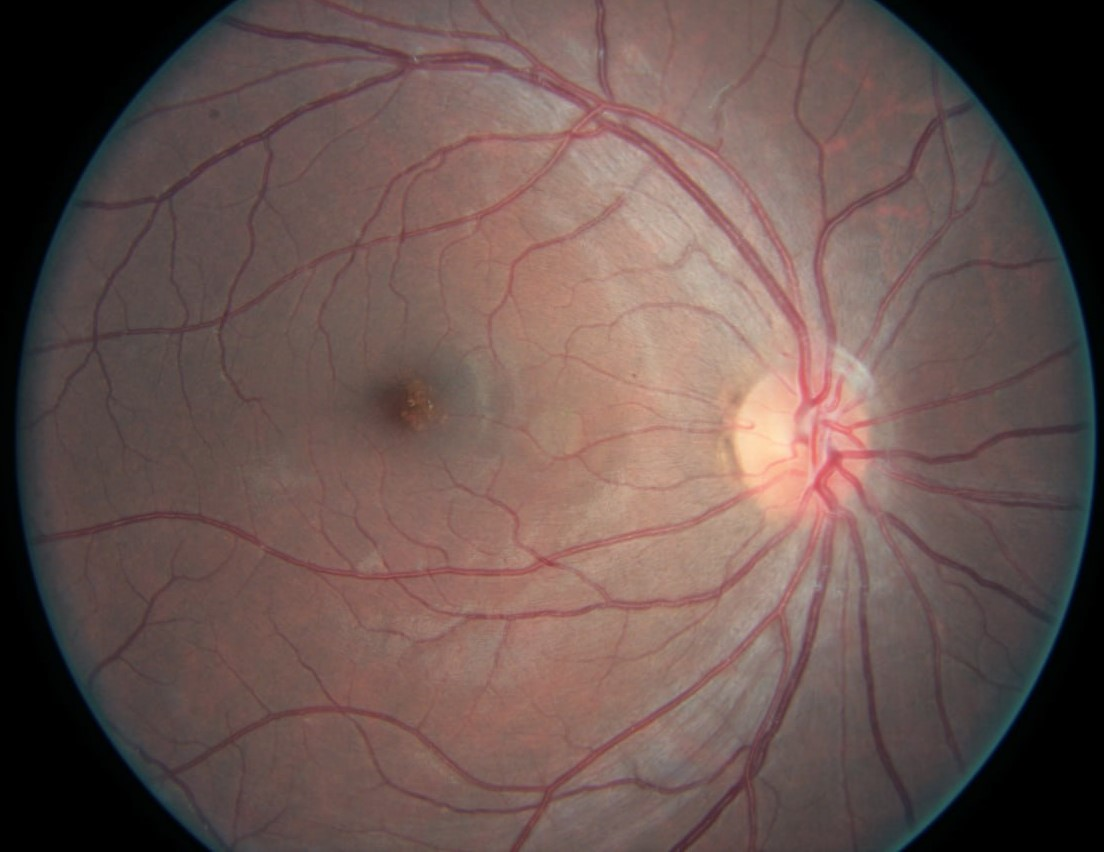
\includegraphics[width=\textwidth, height=0.2\textheight]{figures/chapter6/similar/5997_left.jpg}
            \caption{Grade 0}
         \end{subfigure}
         \hfill
         \begin{subfigure}[b]{0.32\textwidth}
            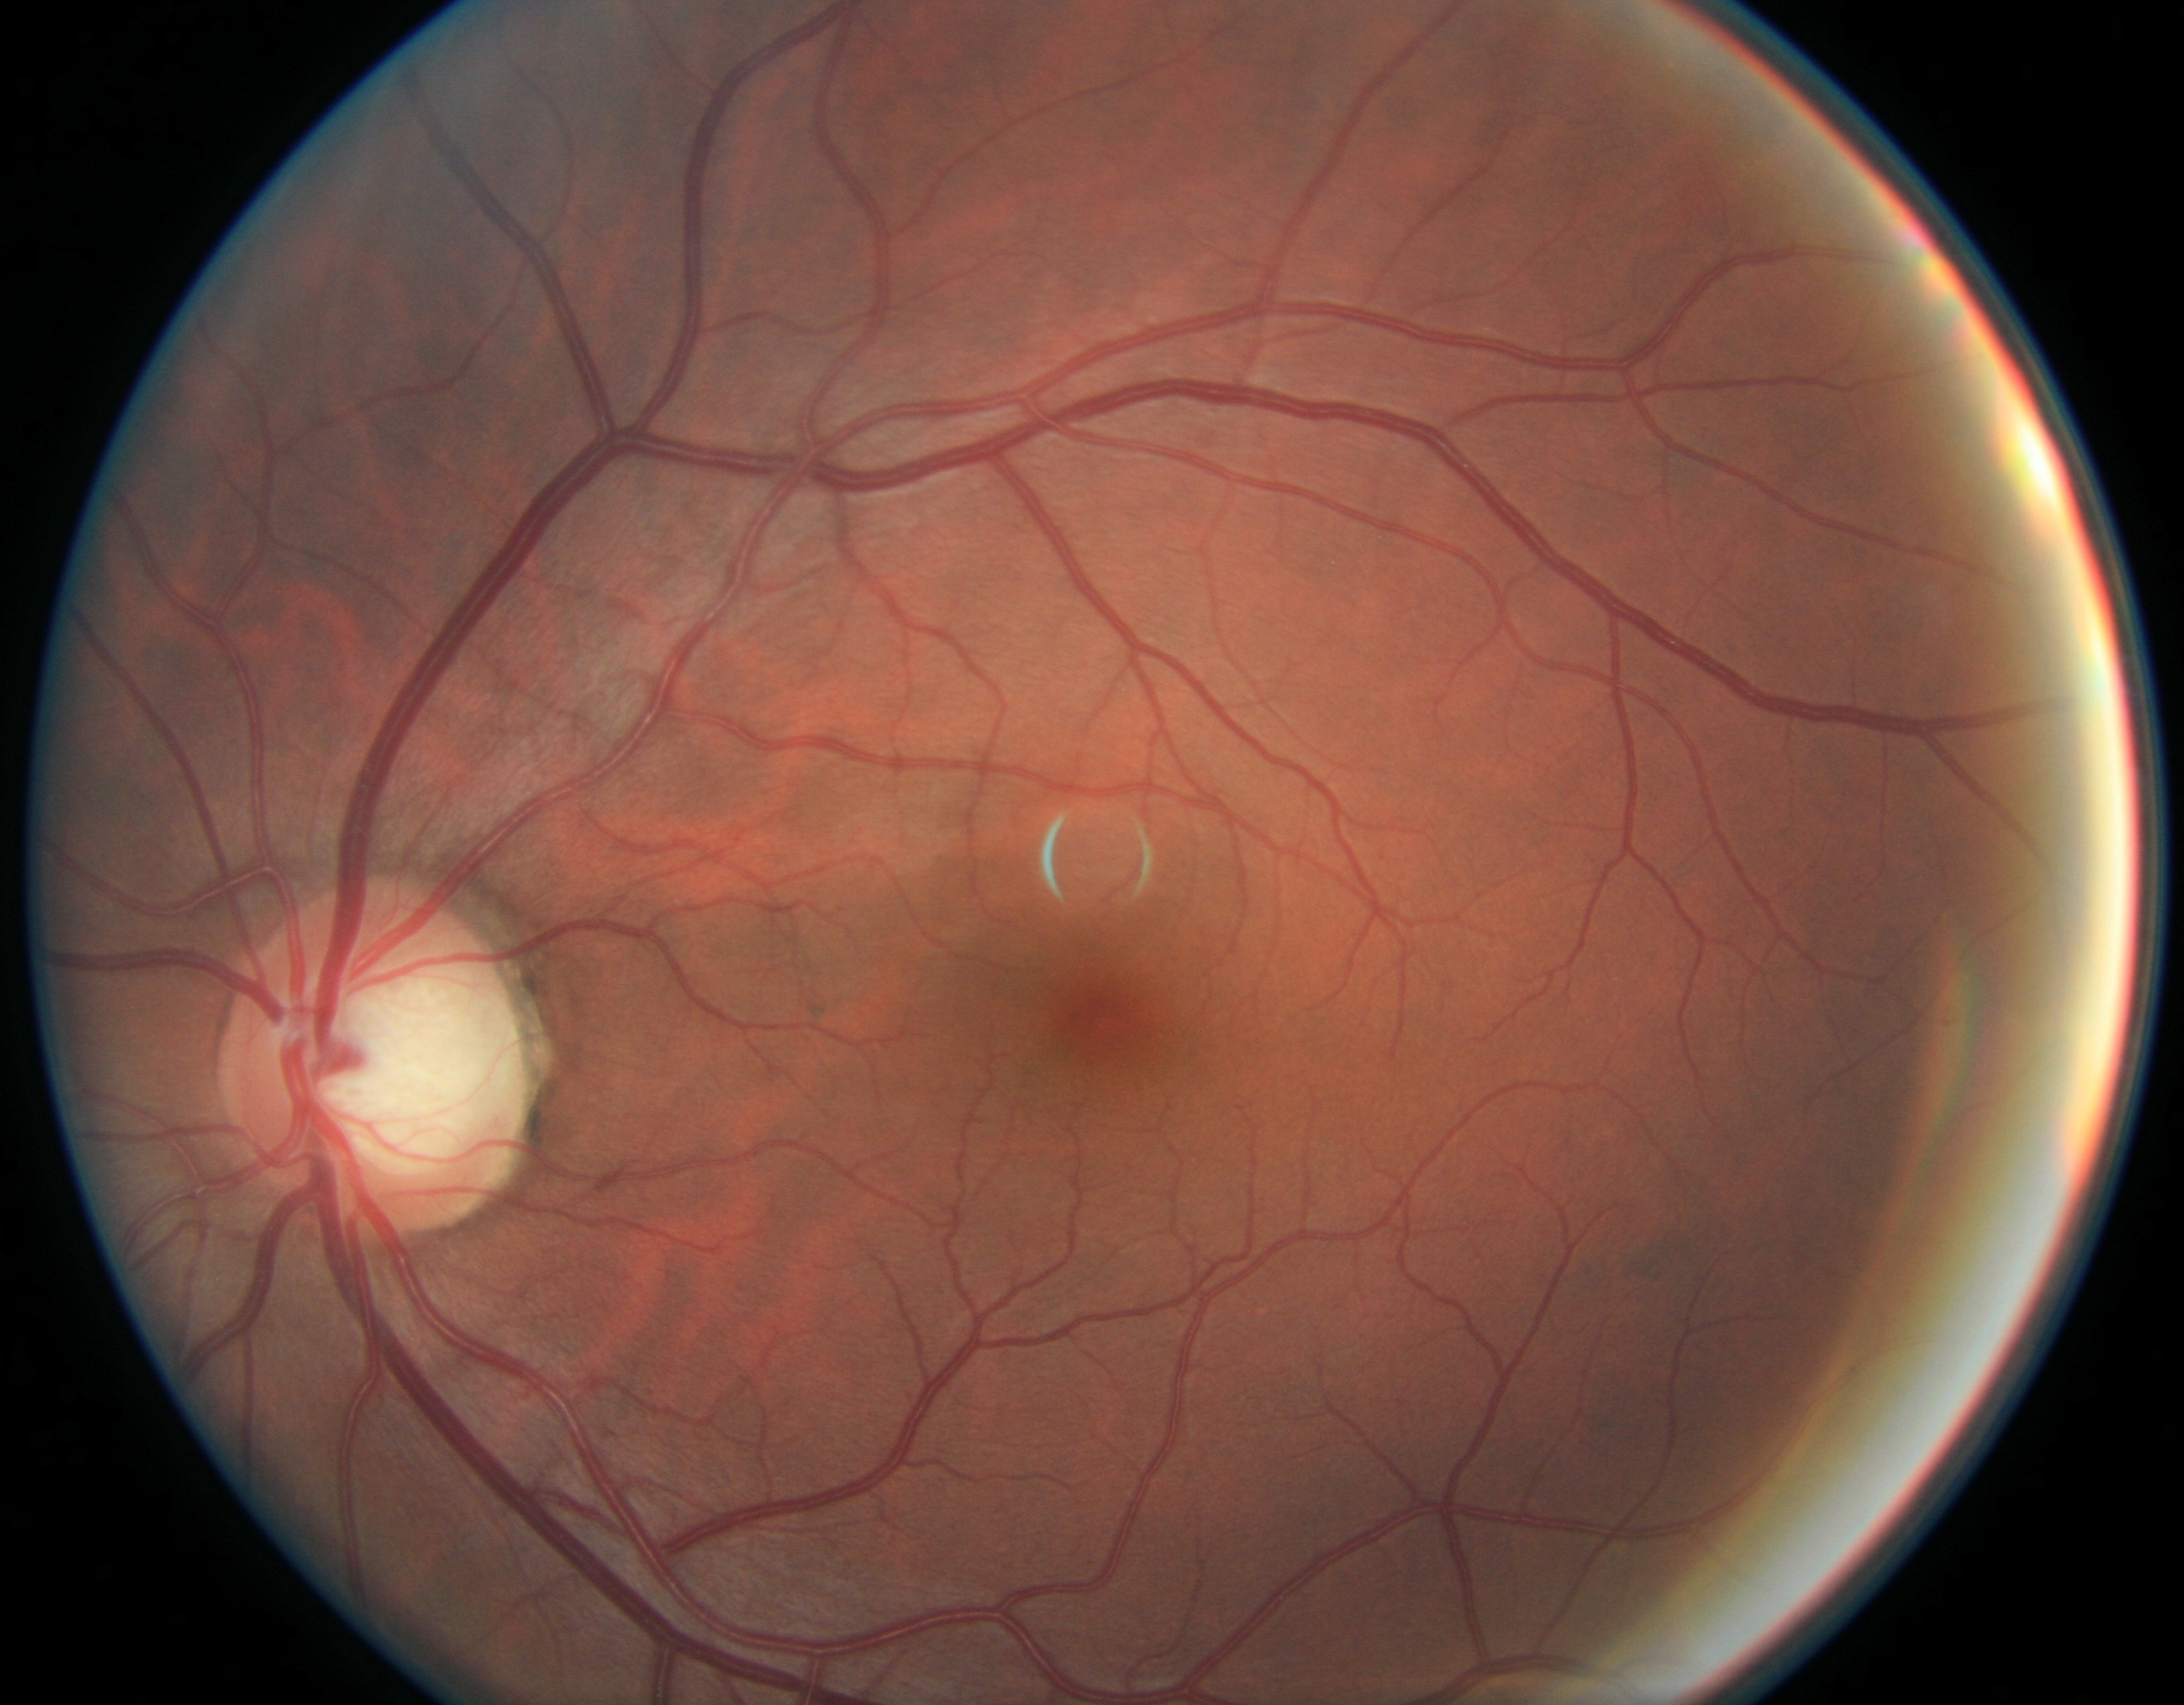
\includegraphics[width=\textwidth, height=0.2\textheight]{figures/chapter6/similar/10861_right.jpeg}
            \caption{Grade 0}
        \end{subfigure}
        \hfill
        \begin{subfigure}[b]{0.32\textwidth}
            \centering
            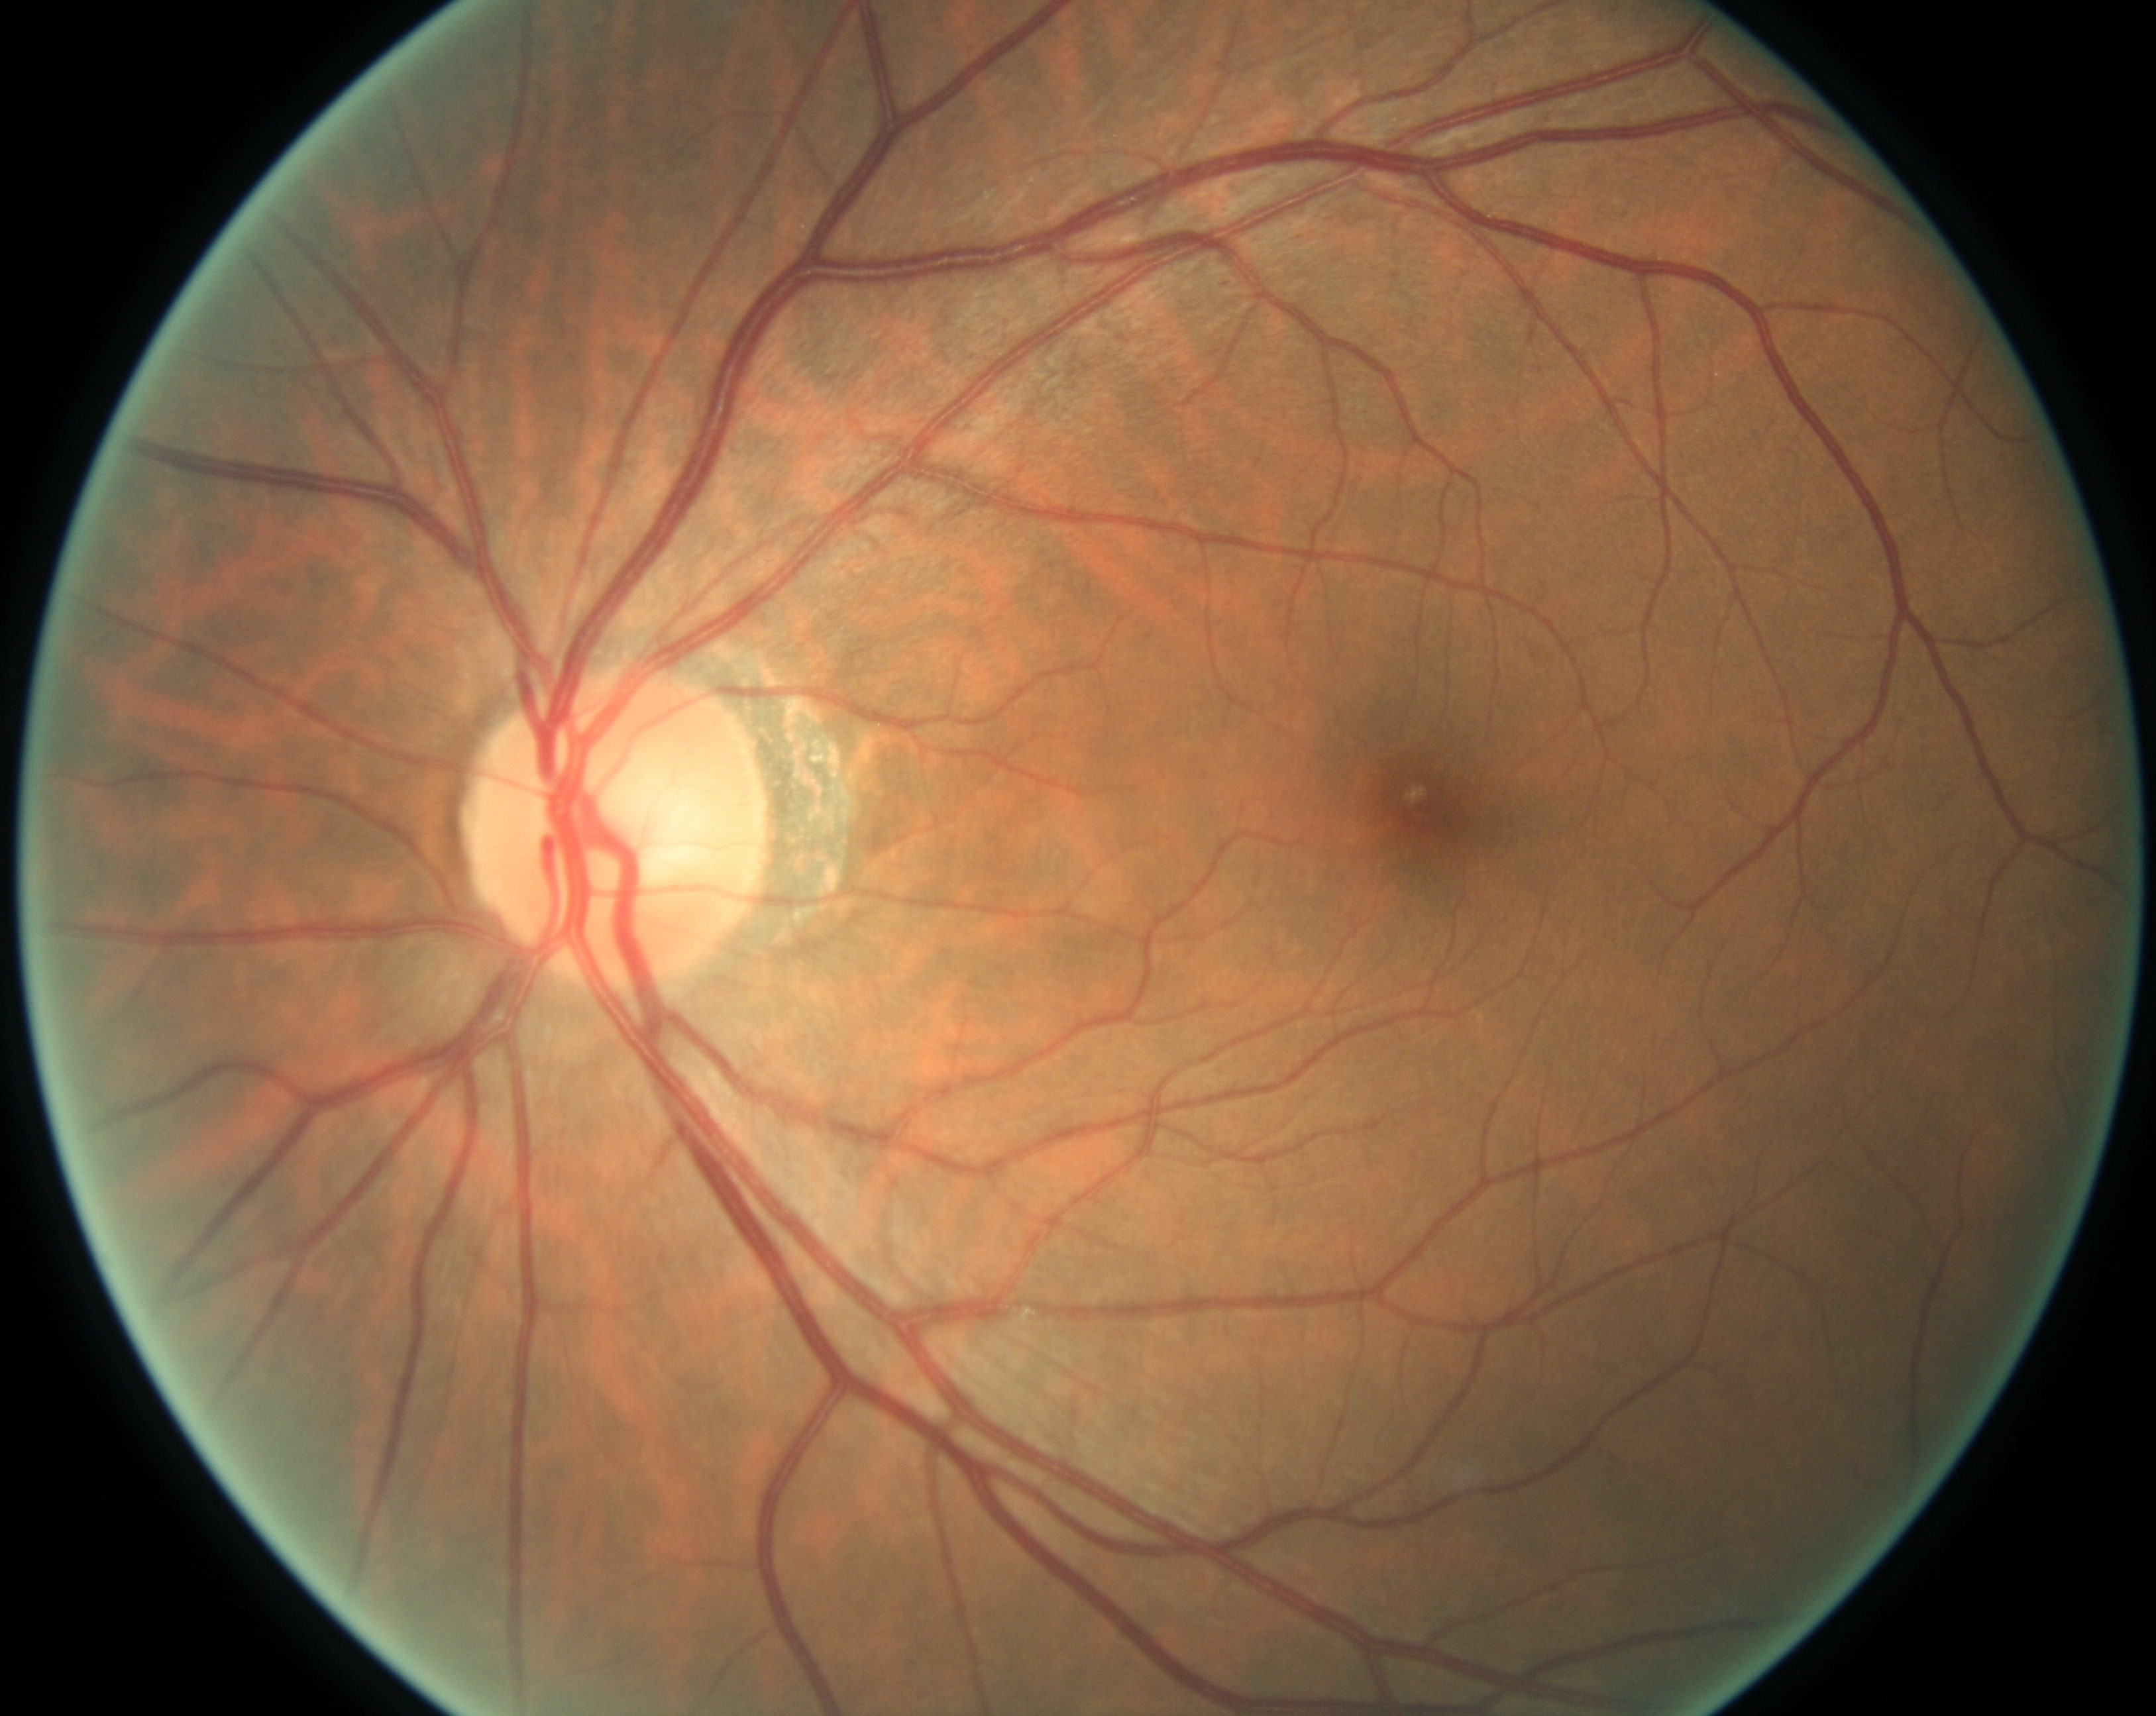
\includegraphics[width=\textwidth, height=0.2\textheight]{figures/chapter6/similar/1669_right.jpeg}
            \caption{Grade 1}
         \end{subfigure}
    \end{subfigure}

    \caption{Two instances (one per row) of retrieval of the two most similar images to a given one (leftmost image), measuring similarity as the distance between 96-dimensional embeddings using cosine distance.}
    \label{fig:semantic_search}
    \centering
\end{figure}

\Cref{fig:semantic_search} shows the result of applying this technique to find the two images in the train set most similar to a base image from the test set, by using cosine distance to measure the distance between embeddings. We found that in 80.49\% of the cases, the image recovered as the closest one using cosine distance has the same grading as the original one and is within one level in 93\% of the cases.

As one might expect, there is an inverse correlation between the distance of the most similar image to the base and both having the same label ($\rho = -0.21$). In fact, an increase of the cosine distance between both images of \( 0.01 \), reduces the probability of both having the same grade by 50.39\% on average. 

Surprisingly, given the robustness of k-NN to the choice of metrics, we have found that different distance functions retrieved generally different images and the measured similarity of a given image can significantly vary between metrics. For example, we found that the closest image according to the cosine distance only was between the top 5 closest images according to the Euclidean distance in 38.53\% of cases. 

%----------------------------------------------------------
%
\section{Experiments and results}
\label{sec:experiments}
%
%----------------------------------------------------------

Two preliminary experiments have been conducted with the collaboration of an ophthalmologist with experience in the treatment of retinal diseases. 

The purpose of the first experiment is to check whether the similarity computed from the image embeddings is consistent with the specialist's intuition of similarity when analyzing the same images. To this end, we show the specialist 1 unlabeled base image from the test set and 5 labeled images from the training set. 

We selected the 5 images from the training set according to their similarity to the test image so that the most similar image and one in the first 4 quantiles  appear. We then asked the specialist to sort the images from the training set in order of similarity to the base image. The specialist can view all the images as many times as she wants with no time limit. This process was repeated 10 times with 10 different images from the test set. 

At the beginning of the experiment, the specialist asked what was exactly meant by ``similarity between images''. There are many criteria that can be taken into consideration: same eye (right or left), similar age of the patient, same type of lesions, same degree of DR development, images made by the same type of imaging device… 

As our neural network calculates the embeddings in the context of a system to diagnose the degree of DR, we instructed the specialist to only take into consideration lesions related to the diagnosis of that disease. Once the similarity criterion was set, the specialist made us realize that she could not sort the images corresponding to healthy eyes, as none of them had lesions. After analyzing the situation, we asked the specialist to group the images according to their similarity to the test image, but without having to order the images in the same group.

% Colorear
\begin{table}[tb]
\centering
\footnotesize
\resizebox{\columnwidth}{!}{
\begin{tabular}{|c|c|c|c|c|} 
\hline
Base & Specialist order & Embeddings order \\ 
\hline\hline
1935l  & \{1831l 4657l 12900l 27782l\} \{28227l\} & 1831l 27782l 12900l 4657l 28227l\\
20883l & \{24656l\} \{16223l 21921r 32104r 35132l\} & 24656l 35132l 21921r 32104r 16223l\\
30476r & \{11219r\} \{13843r 20464l 25222r 32358l\} & 11219r 25222r 13843r 32358l 20464l\\
31466l & \{24711r 29906r 33469l\} \{30919l\} \{10047r\} & 29906r 24711r 33469l 30919l 10047r\\
36651r & \{27153r\} \{13714r 13312l 3395r\} & 27153r 13312l 13714r 6788l 3395r\\
37151r & \{33251r\} \{329l 6569r 29141r\}  & 33251r 29141r 6569r 329l 31428l\\ 
38582r & \{7487l\} \{26381l 27973l\} \{28227l\} \{17221l\} & 7487l 27973l 26381l 17221l 28227l\\
\hline
\end{tabular}
}
\caption{Summary of the results of experiment 1. The first column contains the IDs of the base images. The second column shows the specialist's order (no order is assumed within each set). The last column shows the order according to the cosine similarity and the embeddings. Images 6788l and 31428l were discarded by the specialist due to their quality.}
\label{tab:exp1}
\end{table}

Of the 10 test images analyzed, 3 were discarded because they did not have adequate quality for diagnosis. The results of the other 7 images are shown in \Cref{tab:exp1}. In most cases, the specialist grouped the images into 2 or 3 sets using the type and number of lesions present in each image as the main criterion (her diagnosis of the degree of RD did not always match the image label). These sets should be considered as equivalence classes with no internal order but linearly ordered with respect to its similarity with the base image.

To measure the agreement between the expert's similarity ranking \[ \{ d^{(1)}_1, \dots, d^{(1)}_{n_{1}} \}, \dots, \{ d^{(m)}_1 \dots, d^{(m)}_{n_{m}} \} \]  with the order retrieved from the embeddings \( \mathcal{O} = d^{i_1}_{j_1} < d^{i_2}_{j_2} < \dots < d^{i_l}_{j_l} \), we define the cost of a transposition as \( c(d^{(i_1)}_{j_1}, d^{(i_2)}_{j_2}) = \|i_1 - i_2\| \) and calculate the sequence of transpositions of minimum cost transforming the order \( d^{(1)}_1 < d^{(1)}_2 < \dots < d^{(1)}_{n_{1}} < d^{(2)}_1 < \dots < d^{(m)}_{n_{m}}\) into \( \mathcal{O} \). 

We found this distance to be \( 0 \) in all but one case. Notably, the image retrieved as the most similar one using the embeddings is classified by the expert in the group of the most similar images in all cases, which sustains the claim that our strategy retrieves diagnostically similar images.

The purpose of the second experiment is to make a preliminary study of the usefulness and quality of the retrieved images to help the specialist in her diagnosis. To do this, we again showed the specialist the same 7 base images from the previous experiment and for each of them we followed the following protocol: (1) ask for an initial diagnosis of the image, (2) show the two most similar labeled images from the training set, (3) ask the specialist if she thought they were similar to the base image, (4) ask the specialist if it was useful to be able to see those images, and (5) ask if, in view of those images, she wanted to modify her initial diagnosis.

\begin{table}[tb]
\centering
\small
\begin{tabular}{|c|c|c|c|c|c|} 
\hline
Base & Diagnosis & Retr. tags & Similar? & Useful? & Modify diagnosis?\\
\hline\hline
1935r  & 0 & 0 0 & yes & yes & no \\	
20883l & 2 & 3 2 & yes &	yes & no \\
30476r & 3 & 3 3 & yes &	yes & no \\
31466l & 0 & 0 0 & yes & yes & no \\
36651r & 2 & 3 2 & no  & no  & no \\	
37151r & 1 & 2 1 & yes & yes & no \\	
38582r & 0 & 0 0 & yes & yes & no \\	
\hline
\end{tabular}
\caption{Summary of the results of experiment 2. The first 2 columns contain the ID of the base image to be diagnosed and its initial diagnosis. The third column show the labels of the 2 most similar images retrieved. The last 3 columns show, respectively, whether the specialist considered the retrieved images to be similar to the original one, whether being able to view those images was useful and whether, after viewing the images, she wanted to modify her initial diagnosis.}
\label{tab:exp2}
\end{table}

The results of the experiment are collected in the \Cref{tab:exp2}. The initial diagnosis of the specialist always corresponds to the label of one of the images retrieved using the embedding-based similarity and never differs by more than one degree from the other. Furthermore, in none of the cases are images of diseased eyes retrieved from healthy eyes or vice versa. All retrieved images were considered similar to the originals, except in the case of image 36651 in which the specialist indicated that the retrieved images had different type of lesions. In all other cases, the specialist considered that being able to view those similar images could be helpful for diagnostic support. In no case did the specialist modify her initial diagnosis.

Asked about the possibility of modifying the diagnosis if the system retrieved images with very different labels, the specialist said that she would continue to rely on her judgment unless the system could provide a really convincing explanation. Finally, asked about her overall impressions, she told us that she had been surprised by the system's ability to find similar images and that this feature could be useful for residents.